\documentclass{article}

% set font encoding for PDFLaTeX or XeLaTeX
\usepackage{ifxetex}
\ifxetex
  \usepackage{fontspec}
\else
  \usepackage[T1]{fontenc}
  \usepackage[utf8]{inputenc}
  \usepackage{lmodern}
   \usepackage{graphicx}
  \usepackage{float}
\fi

% used in maketitle
\title{Title of Document}
\author{Name of Author}

% Enable SageTeX to run SageMath code right inside this LaTeX file.
% documentation: http://mirrors.ctan.org/macros/latex/contrib/sagetex/sagetexpackage.pdf
% \usepackage{sagetex}

\begin{document}
\maketitle
\section{Código}
\begin{verbatim}


function funcsx(theta) result(x)
    double precision, intent(in) ::theta
    double precision             ::x
    double precision, parameter :: rs=1.496d8
    x=rs*dcos(theta)
  end function funcsx

  function funcsy(theta) result(y)
    double precision, intent(in) ::theta
    double precision             :: y
    double precision, parameter :: rs=1.496d8
    y=rs*dsin(theta)
  end function funcsy
  
subroutine luna(xl,yl,theta,thetal,rl,rs)
double precision, intent(in):: thetal,theta,rs
double precision, intent(out):: xl,yl,rl
rl=rs/4.0d0

xl=(rs*(dcos(theta)))+(rl*(dcos(thetal)))
yl=(rs*(dsin(theta)))+(rl*(dsin(thetal)))
end subroutine luna

  
!inciamos el programa
  program  stl
  implicit none
  !declaramos Constantes en DP
  !recuerda quela d(número) indicará la potencia a la que se
  !encuentra el número
  !Tomaremos en cuenta el tiempo que toma el movimiento de 
  !traslacion de la luna al igual que el de la tierra
  
  double precision, parameter:: pi=3.1416d0 
  !Tomaremos en cuenta el tiempo que toma el movimiento de 
  !traslacion de la luna al igual que el de la tierra
  double precision, parameter:: lt=27.3217d0, tt=365.26d0
  !declaramos variables
  double precision::theta,funcsy, funcsx,thetal,dia,rad,xl,yl
  double precision::vdl,vds,t,rs,rl
  integer::i
  double precision,dimension(360):: x, y
  double precision,dimension(360)::tx,ty
  rs=1.496d8
  !utilizaremos el operador rad para posteriormente sustituir
  !en lugar de volver a multiplicar por pi y  dividir entre 180
  rad=pi/180.0d0
  !utilizaremos dia para saber cuantos dias transcurren cada radian
  dia=tt/(360.0d0*rad)
  !las variables siguientes se utilizaran para saber 
  !cual es el recorrido de la luna y el sol cada radian
  vdl=2.0d0*(pi/lt)
  vds=2.0d0*(pi/tt)
  
open(1, file= 'stl.dat' , status ='unknown')
open(2, file= 'st.dat', status = 'unknown')
  do i=1,360,1
     t=dble(i)
     theta=t*vds
     thetal=t*vdl
     !lo anterior para calcular la posicion en radianes(por lo estipulado al inicio)
     !igual que en el programa anterior, ponemos los resultados de la
     !función estipulada en el inicio 
     x(i)=funcsx(theta)
     y(i)=funcsy(theta)
     !llamamos a la subrutina para calcular la posicion de la luna
     !respecto al sol
     call luna(xl,yl,theta,thetal,rl,rs)
     tx(i)=xl
     ty(i)=yl
     write(1,*) tx(i) , ty(i)
     write(1,*) ''
     write(2,*) x(i) , y(i)
     write(2,*) ''
     
     end do
     close(1)
     close(2)
end program stl
!






  
  
  !
!! actividad6.f90
!! 
!! Made by (David Eduardo Hernandez Sanchez)
!! Login   <edyhndz7@ltsp166.example.com>
!! 
!! Started on  Mon Nov 27 11:07:58 2017 David Eduardo Hernandez Sanchez
!! Last update Time-stamp: <2010-oct-11.lunes 17:26:15 (calcaneo)>


\end{verbatim}
A continuación se ilustra el resultado obtenido
\begin{figure}[h!]
  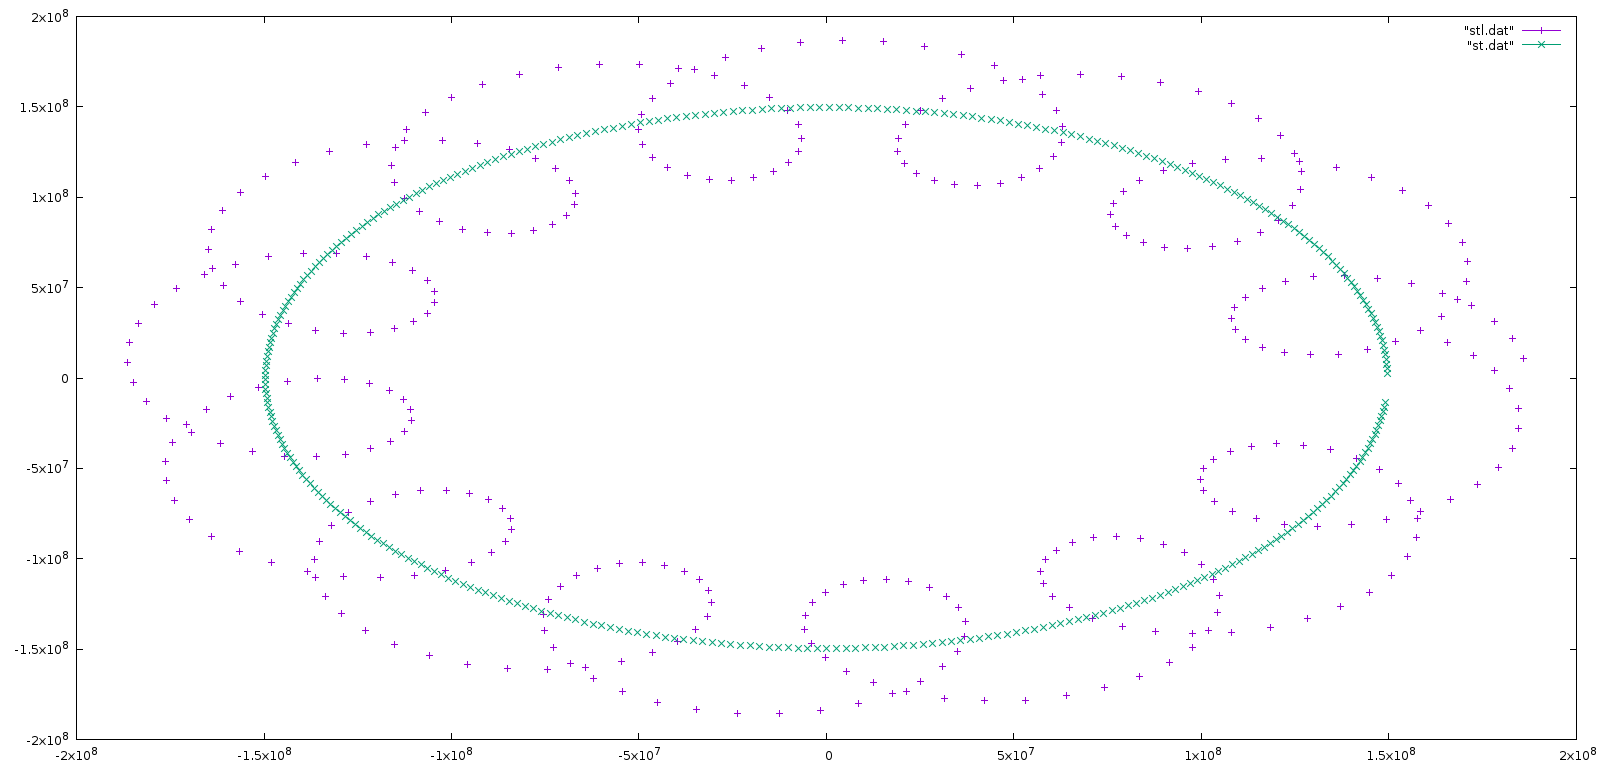
\includegraphics[width=\linewidth]{STL.png}
  \caption{final}
  \label{fig:boat1}
  \end{figure}

\end{document}
